%==============================================================================
% Figure: Meta-Principle Potential Landscape
% Purpose: Multiverse potential with valleys and transition barriers
% Chapter: Ch14 - Genesis Meta-Principle
% Type: Conceptual
%==============================================================================

\begin{figure}[htbp]
  \centering
  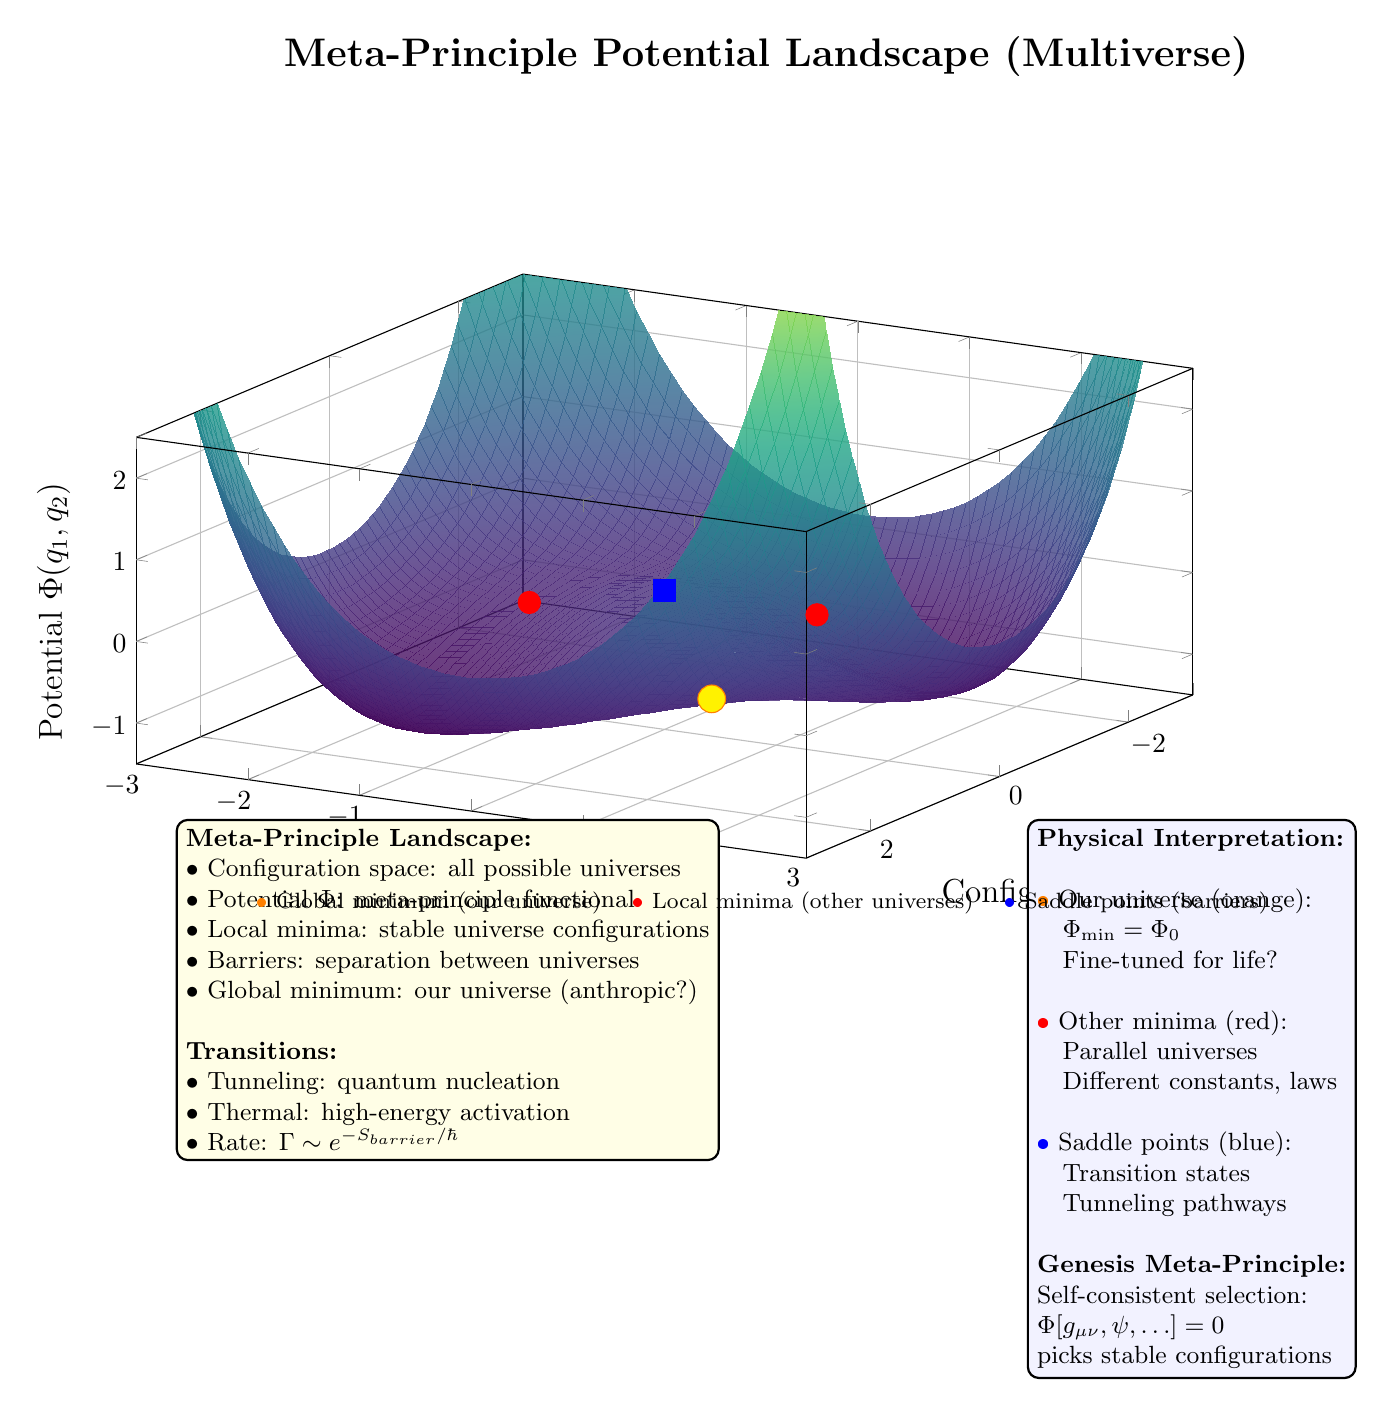
\begin{tikzpicture}[
    scale=1.0
  ]

    \begin{axis}[
      width=15cm,
      height=9cm,
      xlabel={Configuration space $q_1$},
      ylabel={Configuration space $q_2$},
      zlabel={Potential $\Phi(q_1, q_2)$},
      xlabel style={font=\large},
      ylabel style={font=\large},
      zlabel style={font=\large},
      xmin=-3, xmax=3,
      ymin=-3, ymax=3,
      zmin=-1.5, zmax=2.5,
      view={120}{30},
      colormap/viridis,
      shader=interp,
      samples=60,
      domain=-3:3,
      y domain=-3:3,
      grid=major,
      3d box=complete
    ]

      % Complex potential landscape with multiple minima (multiverse)
      \addplot3[
        surf,
        opacity=0.8,
        mesh/interior colormap name=viridis
      ] {
        0.3*(x^2 + y^2 - 4)^2/8 +
        0.4*sin(deg(x))*sin(deg(y)) +
        0.2*exp(-((x-1)^2 + (y-1)^2)/0.5) +
        0.2*exp(-((x+1.5)^2 + (y+0.5)^2)/0.6) +
        0.15*exp(-((x+0.5)^2 + (y-1.5)^2)/0.7) -
        0.8
      };

      % Mark local minima (different universes)
      \addplot3[only marks, mark=*, mark size=4pt, color=red] coordinates {
        (1, 1, -0.6)
        (-1.5, 0.5, -0.5)
        (-0.5, -1.5, -0.4)
      };

      % Mark global minimum (our universe)
      \addplot3[only marks, mark=*, mark size=5pt, color=orange, fill=yellow] coordinates {
        (1, 1, -0.6)
      };

      % Mark saddle point (barrier)
      \addplot3[only marks, mark=square*, mark size=4pt, color=blue] coordinates {
        (0, 0, 0.2)
      };

    \end{axis}

    % Annotations
    \node[anchor=north west, align=left, font=\small, draw=black, fill=yellow!10, rounded corners, thick]
      at (0.5, 0.5) {
      \textbf{Meta-Principle Landscape:} \\
      $\bullet$ Configuration space: all possible universes \\
      $\bullet$ Potential $\Phi$: meta-principle functional \\
      $\bullet$ Local minima: stable universe configurations \\
      $\bullet$ Barriers: separation between universes \\
      $\bullet$ Global minimum: our universe (anthropic?) \\
      \\
      \textbf{Transitions:} \\
      $\bullet$ Tunneling: quantum nucleation \\
      $\bullet$ Thermal: high-energy activation \\
      $\bullet$ Rate: $\Gamma \sim e^{-S_{\text{barrier}}/\hbar}$
    };

    \node[anchor=north east, align=left, font=\small, draw=black, fill=blue!5, rounded corners, thick]
      at (15.5, 0.5) {
      \textbf{Physical Interpretation:} \\
      \\
      \textcolor{orange}{\textbullet} Our universe (orange): \\
      \quad $\Phi_{\min} = \Phi_0$ \\
      \quad Fine-tuned for life? \\
      \\
      \textcolor{red}{\textbullet} Other minima (red): \\
      \quad Parallel universes \\
      \quad Different constants, laws \\
      \\
      \textcolor{blue}{\textbullet} Saddle points (blue): \\
      \quad Transition states \\
      \quad Tunneling pathways \\
      \\
      \textbf{Genesis Meta-Principle:} \\
      Self-consistent selection: \\
      $\Phi[g_{\mu\nu}, \psi, \ldots] = 0$ \\
      picks stable configurations
    };

    % Title
    \node[anchor=south, font=\Large\bfseries] at (8, 9.8) {Meta-Principle Potential Landscape (Multiverse)};

    % Legend symbols
    \node[anchor=north, align=left, font=\footnotesize] at (8, -0.3) {
      \textcolor{orange}{\textbullet} Global minimum (our universe) \quad
      \textcolor{red}{\textbullet} Local minima (other universes) \quad
      \textcolor{blue}{\textbullet} Saddle points (barriers)
    };

  \end{tikzpicture}

  \vspace{0.5cm}

  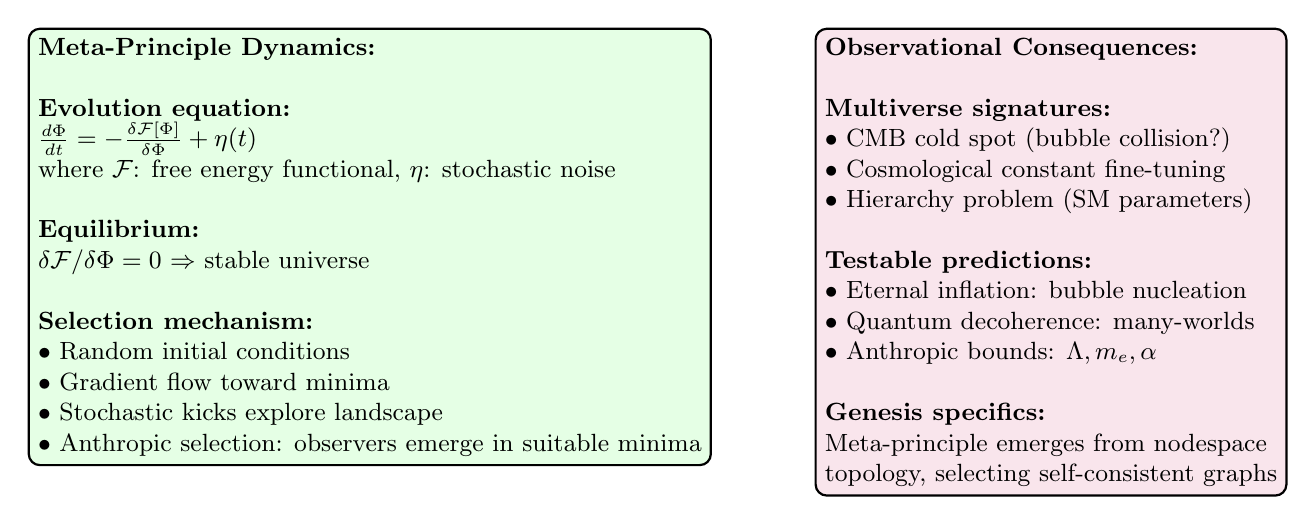
\begin{tikzpicture}
    \node[anchor=north west, align=left, font=\small, draw=black, fill=green!10, rounded corners, thick]
      at (0, 0) {
      \textbf{Meta-Principle Dynamics:} \\
      \\
      \textbf{Evolution equation:} \\
      $\frac{d\Phi}{dt} = -\frac{\delta \mathcal{F}[\Phi]}{\delta \Phi} + \eta(t)$ \\
      where $\mathcal{F}$: free energy functional, $\eta$: stochastic noise \\
      \\
      \textbf{Equilibrium:} \\
      $\delta \mathcal{F}/\delta \Phi = 0$ $\Rightarrow$ stable universe \\
      \\
      \textbf{Selection mechanism:} \\
      $\bullet$ Random initial conditions \\
      $\bullet$ Gradient flow toward minima \\
      $\bullet$ Stochastic kicks explore landscape \\
      $\bullet$ Anthropic selection: observers emerge in suitable minima
    };

    \node[anchor=north east, align=left, font=\small, draw=black, fill=purple!10, rounded corners, thick]
      at (16, 0) {
      \textbf{Observational Consequences:} \\
      \\
      \textbf{Multiverse signatures:} \\
      $\bullet$ CMB cold spot (bubble collision?) \\
      $\bullet$ Cosmological constant fine-tuning \\
      $\bullet$ Hierarchy problem (SM parameters) \\
      \\
      \textbf{Testable predictions:} \\
      $\bullet$ Eternal inflation: bubble nucleation \\
      $\bullet$ Quantum decoherence: many-worlds \\
      $\bullet$ Anthropic bounds: $\Lambda, m_e, \alpha$ \\
      \\
      \textbf{Genesis specifics:} \\
      Meta-principle emerges from nodespace \\
      topology, selecting self-consistent graphs
    };
  \end{tikzpicture}

  \caption{Meta-principle potential landscape in the Genesis framework, representing the space of
    all possible universe configurations. The two configuration coordinates $q_1, q_2$ symbolize
    the infinite-dimensional space of all field configurations, physical constants, and laws. The
    potential $\Phi(q_1, q_2)$ is determined by a meta-principle functional that selects
    self-consistent universes. Local minima (red points) correspond to stable universe configurations
    with different physical laws and constants---a multiverse landscape. The global minimum (orange/yellow)
    may represent our observable universe, possibly selected by anthropic reasoning (observers can
    only exist in suitable minima). Saddle points (blue squares) are barriers between universes;
    transitions occur via quantum tunneling with rate $\Gamma \sim \exp(-S_{\text{barrier}}/\hbar)$
    or thermal activation. The meta-principle evolves the configuration via gradient flow in the
    free energy functional, with stochastic noise allowing exploration of the landscape. In the
    Genesis framework, this landscape emerges from nodespace topology: only self-consistent graph
    structures correspond to stable minima, providing a pre-geometric foundation for universe
    selection. Observable consequences include CMB anomalies from bubble collisions, fine-tuning
    of cosmological constants, and anthropic bounds on fundamental parameters.}
  \label{fig:meta-principle-landscape}
\end{figure}
